% --- [ Control Flow Graph Generation Example ] --------------------------------

\subsection{Control Flow Graph Generation Example}
\label{app:control_flow_graph_generation_example}

The \texttt{ll2dot} tool generates CFGs (in the DOT file format) from LLVM IR assembly files, as described in section~\ref{sec:design_control_flow_analysis}. Using the \texttt{ll2dot} tool, a CFG was generated from the \texttt{main} function of the LLVM IR assembly in listing~\ref{lst:example1_ll}. A textual representation and an image representation of the generated CFG are presented on the left and the right side of figure~\ref{fig:example1_unstructured_cfg} respectively. The image representation was generated using the \texttt{dot}\footnote{Drawing Graphs with dot: \url{http://www.graphviz.org/pdf/dotguide.pdf}} tool of the Graphviz project, by invoking the command \texttt{dot -Tpng main.png main.dot}.

\begin{figure}[htbp]
	\centering
	\begin{subfigure}[ht]{0.38\textwidth}
		\lstinputlisting[language=dot, style=dot]{inc/appendices/ll2dot_example/example1_graphs/main.dot}
	\end{subfigure}
	\qquad
	\begin{subfigure}[ht]{0.20\textwidth}
		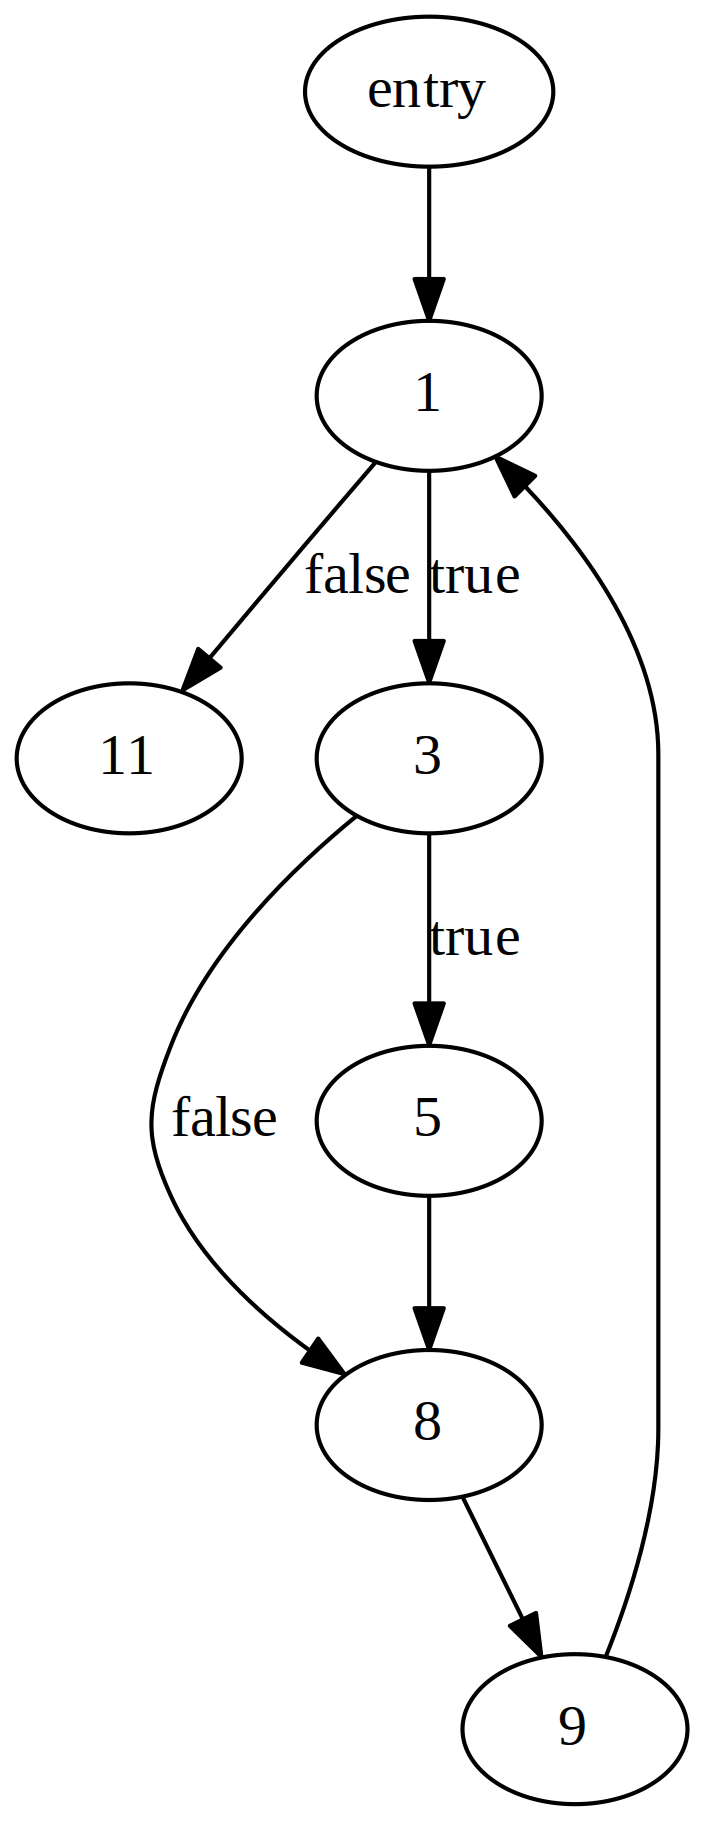
\includegraphics[width=\textwidth]{inc/appendices/ll2dot_example/example1_graphs/main.png}
	\end{subfigure}
	\caption{A textual representation in the DOT file format (left) and an image representation (right) of the CFG which was generated from the \texttt{main} function of the LLVM IR assembly in listing~\ref{lst:example1_ll}, using the \texttt{ll2dot} tool.}
	\label{fig:example1_unstructured_cfg}
\end{figure}
